\documentclass[13pt]{article}
\usepackage{a4wide}
\usepackage[utf8]{inputenc}
\usepackage[T1]{fontenc}
\usepackage[french]{babel}
\usepackage[babel=true]{csquotes} % guillemets français
\usepackage{graphicx}
\graphicspath{{Images/}}
\usepackage{color}
\usepackage{hyperref}
\hypersetup{colorlinks,linkcolor=,urlcolor=blue}
\usepackage{amsmath}
\usepackage{amssymb}


\title{Rapport exercice 2.3}
\author{CHAN CHUN TIM Alan,L3 Informatique}
\begin{document}
\maketitle %
\begin{abstract}
Dans ce rapport je vais vous expliquer mon programme de file en JAVA et en PYTHON 
\end{abstract}
\section{Introduction}
\label{section:Introduction} % pour faire référence à la section ailleurs (\ref{...} voir plus bas)
Dans le cadre de l'UE de programmation concurrente, l'objetif est la création de programmes qui représente une file en PYTHON et en JAVA avec une interfce graphique. Ces étapes seront illustrées par des images et des bouts de code.
\section{Qu'est-ce qu'une file?}
Le principe du FIFO(First In first Out) est la conservation de l'ordre d'entrer lors de la sortie d'articles ou d'entités dans une file, un stock, un contenant. L'illustration du FIFO pourrait en être un tube dans lequel les pièces sortent séquentiellement dans le même ordre qu'elles y sont entrées, comme le montre l'illustration ci-dessous.
\begin{center}
  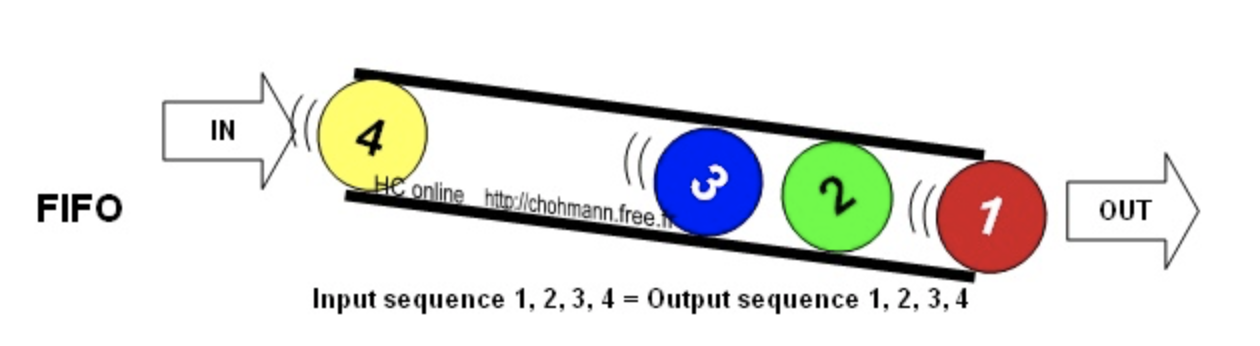
\includegraphics[scale=0.5]{image1.png}
\end{center}
\subsection{Ma classe FIFO}
Ma classe Fifo a pour objectif de supprimer les premiers éléments d'une liste de longueur maximale 20 et minimum 0 et d'ajouter des éléments à la fin de la liste.
De ce fait j'ai créé une fonction remover(qui supprime) et une fonction adder(qui ajoute).
\subsection{Exemple JAVA}

\begin{verbatim}
public synchronized void remover() throws InterruptedException {
        if (o.isEmpty())return;
        while (o.isEmpty())wait();
        Integer k = o.get(0);
        o.remove(0);
        f.Update(o,k,false);
    }
	
public synchronized void adder( int p) throws InterruptedException {
        if (o.size()>19)return;
        o.add(p);
        notifyAll();
        f.Update(o,p,true);
    }
	
\end{verbatim}

\subsection{Exemple PYTHON}
\begin{verbatim}
def remover(self):
        with self.cond:
            while len(self.liste) == 0:
                self.cond.wait();
            val = self.liste.pop(0)
            self.fenetre.update(self.liste,rm=val)
            self.cond.notifyAll()
        
    def adder(self,v):
        with self.cond:
            while len(self.liste) >= 20:
                self.cond.wait()
            self.liste.append(v)
            self.fenetre.update(self.liste,add=v)
            self.cond.notifyAll()
\end{verbatim}
\section{L'utilisation des Threads}
Comme les deux fonctions (adder, remover)doivent être utilisé en parallèle l'utilisation des threads est approprié. Si on décrit le code précédant la fonction remover est en attente tant que la liste est vide (while (o.IsEmpty())wait();) et dans la fonction adder ajoute un élément à la fin de la liste et utilise notifyall()pour changer l'état du thread.

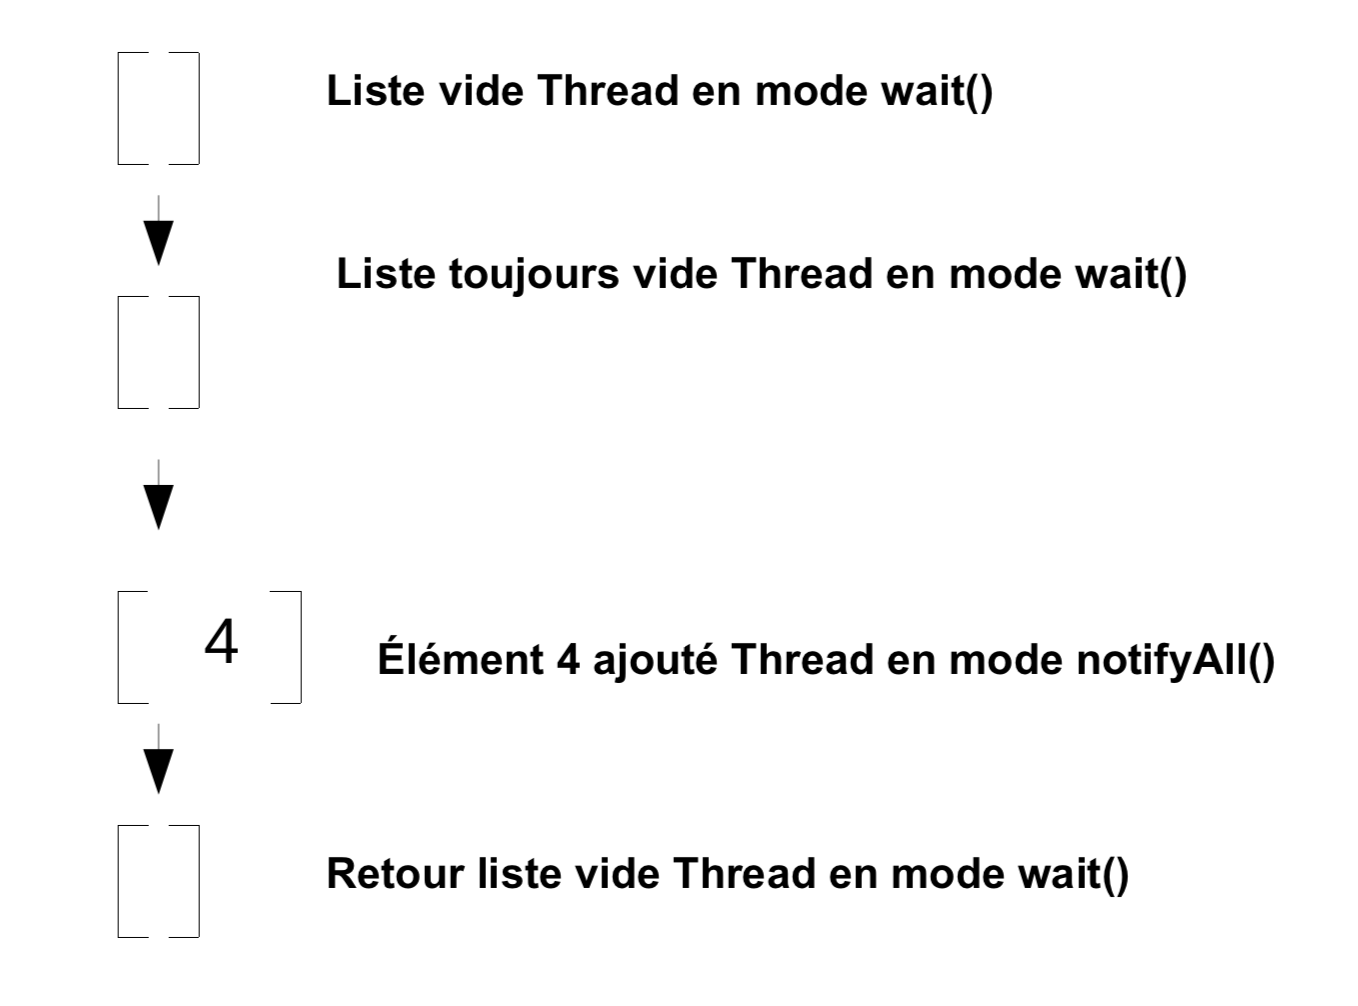
\includegraphics[scale=0.5]{image3.png}

\subsection{Thread Producteur}
La classe ThreadProducteur permet de modéliser un producteur qui dépose des entier compris entre 1 et 100 dans une liste. Le thread a un temps de repos de 300 millisecondes(Thread sleep(300);)en JAVA et un temps 2 secondes en PYTHON. Voici 2 exemples de classe Thread Producteur:

\subsection{Exemple JAVA}
\begin{verbatim}
public void run() {
	      System.out.println("Producteur Commence");
	      try {
	         while(true) {
	        		 int v =(int)(Math.random()*(100-1+1)+1);
	        		 f.adder(v);
	        		 Thread.currentThread();
				 Thread.sleep(300);
	         }
	      } catch (Exception ex) {
	         ex.printStackTrace();
	      }
	 }    
\end{verbatim}
\subsection{Exemple PYTHON}
\begin{verbatim}
def run(self):
        while(True):
            v = random.randint(1, 100)
            self.file.adder(v)
            time.sleep(2)
\end{verbatim}
\subsection{Thread Consommateur}
La classe ThreadCosommateur permet de modéliser un consommateur qui retire des éléments dans la liste. Le thread à un temps de repos de 900 millisecondes en JAVA et un temps de 4 secondes en PYTHON

\subsection{Exemple JAVA}
\begin{verbatim}
public void run() {
	     public void run() {
		      System.out.println("Consumer Started");
		      while(true) {
		      try {
		    	  	
		    	  		f.remover();
		            Thread.currentThread();
					Thread.sleep(900);
		         } catch (Exception ex) {
		            ex.printStackTrace();
		         }
		      }
	   }
\end{verbatim}
\subsection{Exemple PYTHON }
\begin{verbatim}
public void run() {
	     def run(self):
        while True:
            self.file.remover()
            time.sleep(4)
\end{verbatim}
\section{Interface Graphique}
En JAVA pour l'interface graphique j'ai utilisé les packages javas swing, java Awt .
La fonction Update permet de transmettre les informations à la fenêtre. Il gère changement d'attribut pour les valeurs de la liste et gère l'affichage des éléments supprimer et ajouter.\\

\begin{verbatim}
public void Update(List<Integer> l, int k, boolean add)
	{
        String str = "<";
            for(int i = 0; i<l.size() ;i++) {
            str += Integer.toString(l.get(i)); 
            str += (i + 1 < l.size())?" , ":"";
           }
        str += ">";
        txt.setText(str);
		
        if(add) {
          prodTxt.setText("L'élément "+Integer.toString(k)+" a été ajouté.");
        }
        else {
         consTxt.setText("L'élément "+Integer.toString(k)+" a été supprimé.");
        }
        //this.repaint();
    }
\end{verbatim}
\vspace{5mm}
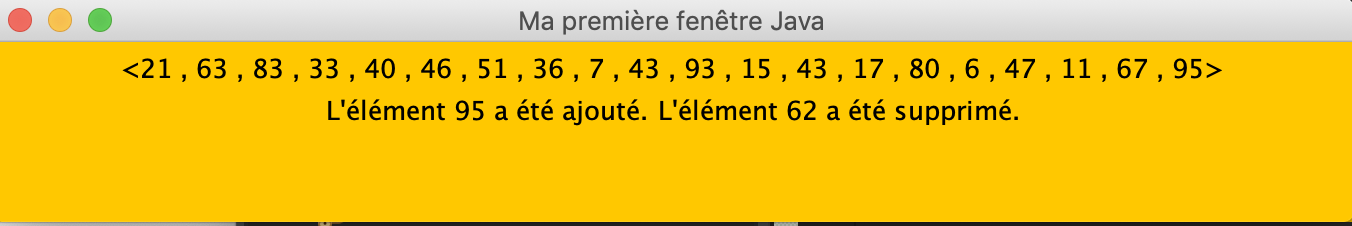
\includegraphics[scale=0.7]{image5.png}
\vspace{5mm}

En PYTHON pour l'interface graphique j'ai utilisé le pakage tinter.
De même La fonction Update permet de transmettre les informations à la fenêtre. Il gère changement d'attribut pour les valeurs de la liste et gère l'affichage des éléments supprimer et ajouter.

\vspace{5mm}
\begin{verbatim}
def update(self,liste,add=None,rm=None):
        self.fileText.set("File = "+str(liste))
        if add != None:
            self.prodText.set("Producteur 0 : "+str(add)+" a été ajouté")
        if rm != None:
            self.consText.set("Consommateur : "+str(rm)+" a été supprimé")
        self.packFen()
\end{verbatim}
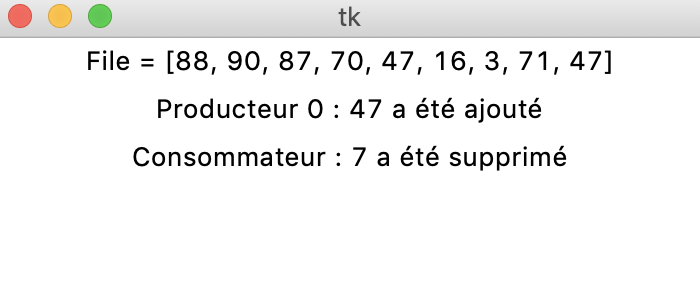
\includegraphics[scale=1.2]{image4.png}
\section{Conclusion}
Pour la création du programme files j'ai créé plusieurs classes(Fifo, fenêtre,Thread Consommateur, Thread Producteur ,main) dans les deux langages. Pour que les deux Threads puissent être utilisé de manière synchroniser l'utilisation de wait et de notifyall est indispensable. Pour l'interface Graphique j'ai utilisé des bibliothèque adaptés pour pouvoir afficher les listes et les éléments qui ont été supprimer et ajouter à la liste.
\section{Annex}
lien java:
\url{https://openclassrooms.com/fr/courses/26832-apprenez-a-programmer-en-java}\\
lien interface graphique java:
\url{https://openclassrooms.com/fr/courses/26832-apprenez-a-programmer-en-java/21973-les-classes-abstraites-et-les-interfaces}
lien interface graphique python :
\url{http://apprendre-python.com/page-tkinter-interface-graphique-python-tutoriel}

\end{document}